%NOTE: COMPILE IN TERMINAL USING LUALATEX
\documentclass[a4paper,8pt]{standalone}

\usepackage{tikz-feynman}
%\usetikzlibrary{external}             %% Load the `external` library
%\tikzexternalize
%\immediate\write18{mkdir -p pgf-img}
%\tikzexternalize[                     %% Activate externalization
%  system call={                       %% Use lualatex in system call
%    lualatex \tikzexternalcheckshellescape -halt-on-error -interaction=batchmode -jobname="\image" "\texsource" || rm "\image.pdf"
%  },
%]

\begin{document}

%\feynmandiagram [horizontal=a to d]{
%    b -- [gluon] c -- [fermion,edge label'=$t$] c1 -- [gluon] b1,
%    c -- [fermion,edge label=$t$] a -- [fermion,edge label=$\bar t$] c1,
%    a -- [scalar,edge label=$H$] d,
%    b -- [opacity=0] b1,
%};

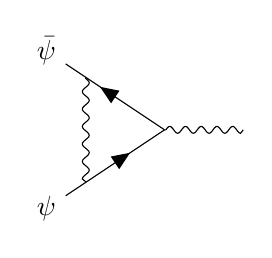
\begin{tikzpicture}
    \begin{feynman}
        \vertex (a1) {$\bar{\psi}$};
        \vertex at ($(a1)+(0.5cm,-0.33cm)$) (a2);
        \vertex[below=1.33cm of a2] (a3);

        \vertex[below=2cm of a1] (b1) {$\psi$};
        \vertex at ($(b1)+(1.5cm,1cm)$) (b2);

        \vertex[right=1cm of b2] (c1);

        \diagram* {
            (a1) -- [anti fermion] (b2) -- [anti fermion] (b1),
            (a2) -- [photon] (a3),
            (b2) -- [photon] (c1),
        };
    \end{feynman}
\end{tikzpicture}


\end{document}
